\chapter{Design and Implementation}
\section{Introduction}
This chapter will discuss in detail the design and implementation of the Blockchain in NDN. It will outline and justify different design choices that were made along the way and also the difficulty they presented/alleviated. 

The Design is sectioned into: The Development Platform, The Data Structure and Content Delivery, which will be discussed in that particular order.
\section{The Development Platform}
\subsection{MiniNDN}
There are a number of tools which can be used to experiment with NDN. These are the following: ndnSIM, Docker and MiniNDN.
MiniNDN is an emulator. It is an extension of mini-net - a networking emulator. On top of mini-net, one can install MiniNDN and all of its modules:Chronosync, PSync, NDN-CXX, NDN-CPP, NFD and NLSR.

There are a couple of reasons why MiniNDN was chosen for this product. Firstly, it is very easy to set up. The knowledge required to get started with MiniNDN is minimal. It is largely based on MiniCCNx which is a fork of  Mininet meaning there are plenty of resources available online in terms of reading material on getting started.

It goes without saying that MiniNDN was also chosen because it is open and free under the GNU General Public License. They also have a Redmine site which tracks and describes all bugs/features as well as a useful mailing list for any developers looking to experiment with the software.

 There are also a number of MiniNDN specific tutorials that have been created by NDN's main coders - Alexander Afanasyev and Ashlesh Gawande. They go into quite a bit of depth regarding different utilities in MiniNDN. Ashlesh's tutorial mainly concerns experiments and topologies where Alex's tutorial goes a bit more in depth regarding node interactions. 
 
 There are drawbacks associated with using MiniNDN also. It is an emulator not a simulator, meaning all of the topologies tested are created in real time - with NLSR convergence happening in real time also. This means that for a portable machine, with an 8th generation hyper-threaded Intel i7 processor, it can take up to 70 seconds for NLSR to converge on a basic 4 node topology. This however scales with CPU performance, so more CPU power should result in much lower convergence times. 
 
 As well as that, when defining topologies or writing experiments, the emulator must be reinstalled every time in order for these changes to be recognized.
 
 MiniNDN works by creating an NDN container around nodes in a mininet simulator. Each node then runs an instance of NFD and NLSR. The user can then configure topologies - including amount of nodes, nodes' identities and adjacencies. As well as that the user can set parameters for hyperbolic routing which NLSR can run on if set in the configuration file. 
 
 As well as this, MiniNDN is useful because we can run different programs on nodes without having to use the python experiments and reinstall MiniNDN every time we alter an experiment. Each node can run an xterm in the background by using the command $"{<}node{>} \; xterm \; \& "$ after which the user can export the home folder for each node and run any of the sample programs from the NDN libraries or indeed write their own. 
\begin{figure}

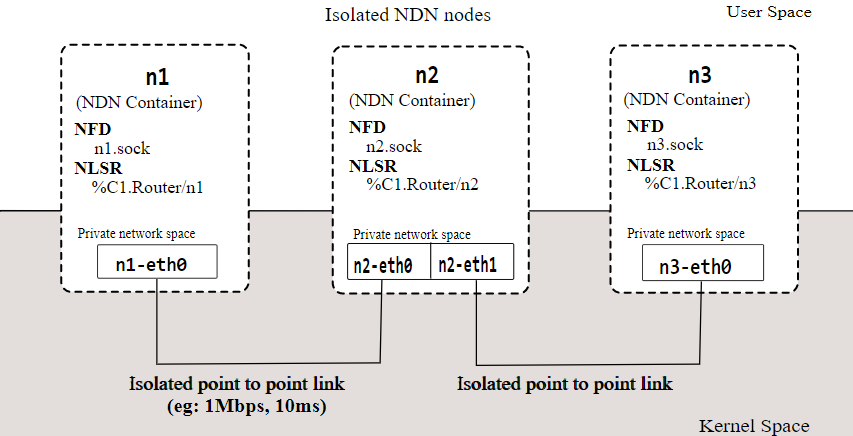
\includegraphics[width=6in]{minindn}
\caption{Basic MiniNDN architecture}
\end{figure}

\section{The Data Structure}
There are two data structures which were designed for the scope of this projects. These are the PibBlock and PibBlockchain. The PibBlockchain maintains a vector of hashed PibBlocks. It can return, at an index, a particular hashed block. It is maintained by the Public Information Base. 

The PibBlock class deals with the Certificates. It stores all information about a certificate as well as its version and the hash of the previous block.
\subsection{Public Information Base Block}
This is the basic building block of the PibBlockchain. It contains the current block's hash, certificate, version and timestamp as well as the previous block's hash. Mining the block is also done in the block class. The difficulty of the block mining is determined by the proof of work algorithm which takes in a a difficulty argument which determines how many zeroes need to be mined by the algorithm until a block is valid. For the purposes and scope of this project however, this algorithm wasn't fully implemented. 

The PibBlocks's constructor returns a pointer to a PibBlock's location in memory. For the initial Block, the PibBlock constructor takes no arguments and creates the genesis block which is based on a nonce cert. This is because we need to have an initial block with which we can hash the rest of the blocks. This bit of design wasn't particularly necessary as mentioned previously, the hashing algorithm wasn't implemented fully in the first place. 

Because the PibBlock class doesn't use smart pointers(more on this later), the class must have an explicitly defined destructor. In this destructor, all of the PibBlock's components are deleted. It is however important to note that the PibBlock's destructor doesn't correlate to the PibBlock's invalidator. Once created, a PibBlock cannot be destroyed or it will invalidate the whole Blockchain. Instead, there is an invalidator function, which simply sets the version of a PibBlock to 0 to imply that it has been invalidated. If the same certificate needs to be validated again, it must go through the whole proof of work process and be hashed to a new block with a version number 1.

Perhaps the most important design element of the PibBlock was the displaying of information. Early iterations would have each PibBlock copy a certificate onto a new certificate instance before adding the Block to the Blockchain. This proved disastrous as NFD does not allow certificates that haven't been signed by the KeyChain to exist, and if any are found the NDN network is shut down immediately.
\subsection{Public Information Base Blockchain}

Public Information Base(PIB) - This is the public key infrastructure hierarchy where identities are stored. Each identity in a network contains within it a default key and a default certificate. The counterpart private key information is stored in the Trusted Platform Module(TPM). We do not concern ourselves with the TPM as we only need the public keys to verify a node's signature. This is standard security procedure in any network. 

The PIB class in the NDN-CXX library is responsible for creating and publishing certificates. The design suggested by Dr. Weber was to create a wrapper so that any time a certificate is created, we could simply add it to the blockchain. Then the miner nodes could verify it and publish the given information. This however proved challenging in a number of ways. 

The first issue I encountered had to do with instancing. Because we needn't necessarily have only one instance of a PIB, we have to make sure that each PIB's certificates go in that specific PIB's Blockchain. This is precisely why Alexander Afanasyev has designed the PIB class in a way that one cannot instantiate a Trusted Platform Module(TPM) outside the PIB class i.e. the constructor for the PIB is the only place where the TPM is also constructed. This means that we cannot have a PIB be matched with a TPM that isn't its counter part. I aimed to achieve the same goal. I did this by looking outside of the PIB class. The PIB class is instantiated and governed by the KeyChain class. This in turn means that the KeyChain class instantiates both the PIB and the TPM. This is why I tried to make the constructor for the PibBlockchain data type to use as an argument the KeyChain's address meaning it would be instantiated in the KeyChain with code that looks something like "PibBlockchain certChain = new PibBlockchain(this);"

However, the PIB Blockchain was comprised of blocks or PibBlocks, which were a separate data structure which made use of the Certificates class in order to store certificates or indeed to be able to parse them at all in the first place. Because PibBlock inherited from Certificates, and PibBlockchain inherited from PibBlock and KeyChain inherited from both PibBlockchain and Certificates, there was suddenly a circular dependency which could not be broken without completely scrapping the PibBlockchain constructor design which takes a pointer to the KeyChain as an argument. 

\begin{figure}
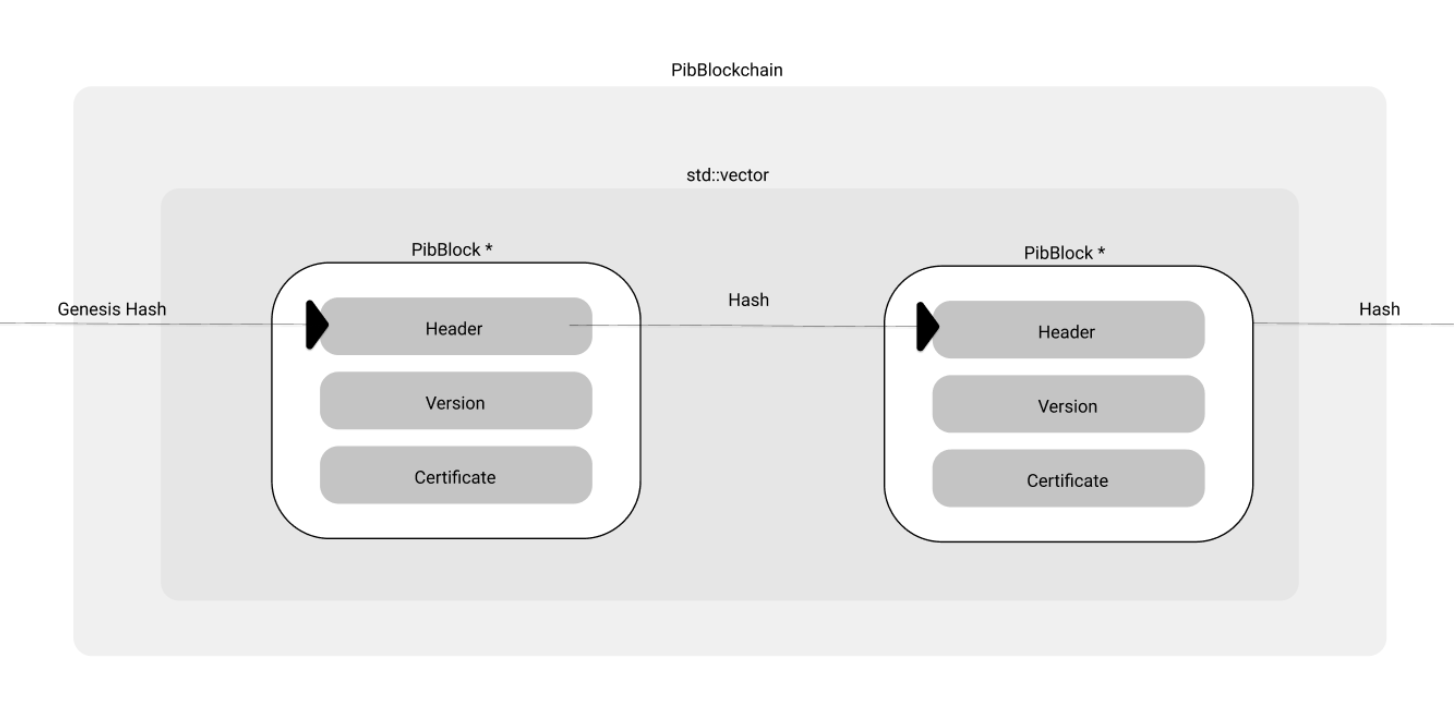
\includegraphics[width=6in]{pibblockchain.png}
\caption{This figure shows how PibBlockchain interacts with NDN and the std library}
\end{figure}

This is where Dr. Weber's original "wrapper" idea came to mind and to good use. Instead of having to worry about the KeyChain pointing to the correct PibBlockchain for each PIB, we could just instead make a mutable PibBlockchain in the PIB class which would work on the exact same principle as Alex Afanasyev's idea to instantiate the TPM in the PIB. We simply do the same thing with the PibBlockchain and instantiate it in the PIB. This way, we no longer have to worry having mismatched PIB and Blockchain. 

Blocks on the other hand weren't at all a concern when it came to creating instances of the Blockchain. The purpose of the PibBlock class is twofold: Firstly, to encapsulate all of the data from each Certificate and secondly, to do all of the "heavy lifting". What this means is that the PibBlock class is responsible for the hashing of each block. 

Of course this doesn't mean that there isn't a concern about which blocks go in which Blockchain. However, blocks are only created when Certificates are created. Certificates are created in the KeyChain.cpp. This means that each KeyChain has only one PibBlockchain to work with, because each KeyChain only instantiates one PIB. One PIB = One PibBlockchain. Therefore if we create PibBlocks in the KeyChain they will inherently be PibBlockchain specific and will be out of scope for any other KeyChains or PibBlockchains. This inherent property of C++ and indeed all object oriented programming made the challenge of making sure that each PibBlock is added to the correct Blockchain very simple.

"Within C++, there is a much smaller and clearer language struggling to get out" - Bjarne Soustroup[cit needed]
\\


Now that the allocation of PibBlocks to PibBlockchains was completed, and there were no longer any circular dependencies allowing for the code to be added to the security code hierarchy in NDN-CXX. \par 

Shortly after adding the code to the project, it became evident that the solution wouldn't work in its current form. That is because the NDN Team have developed a pretty robust automatic Certificate Authority. I found this out when I realized that my PibBlock data structure was parsing certificates being created, allocating new memory for them and then copying the certificate. The problem with this approach is that the copied certificates have not been authorised by the Certificate Authority. This is why when running the simulation, it would abruptly exit. 


\begin{figure}
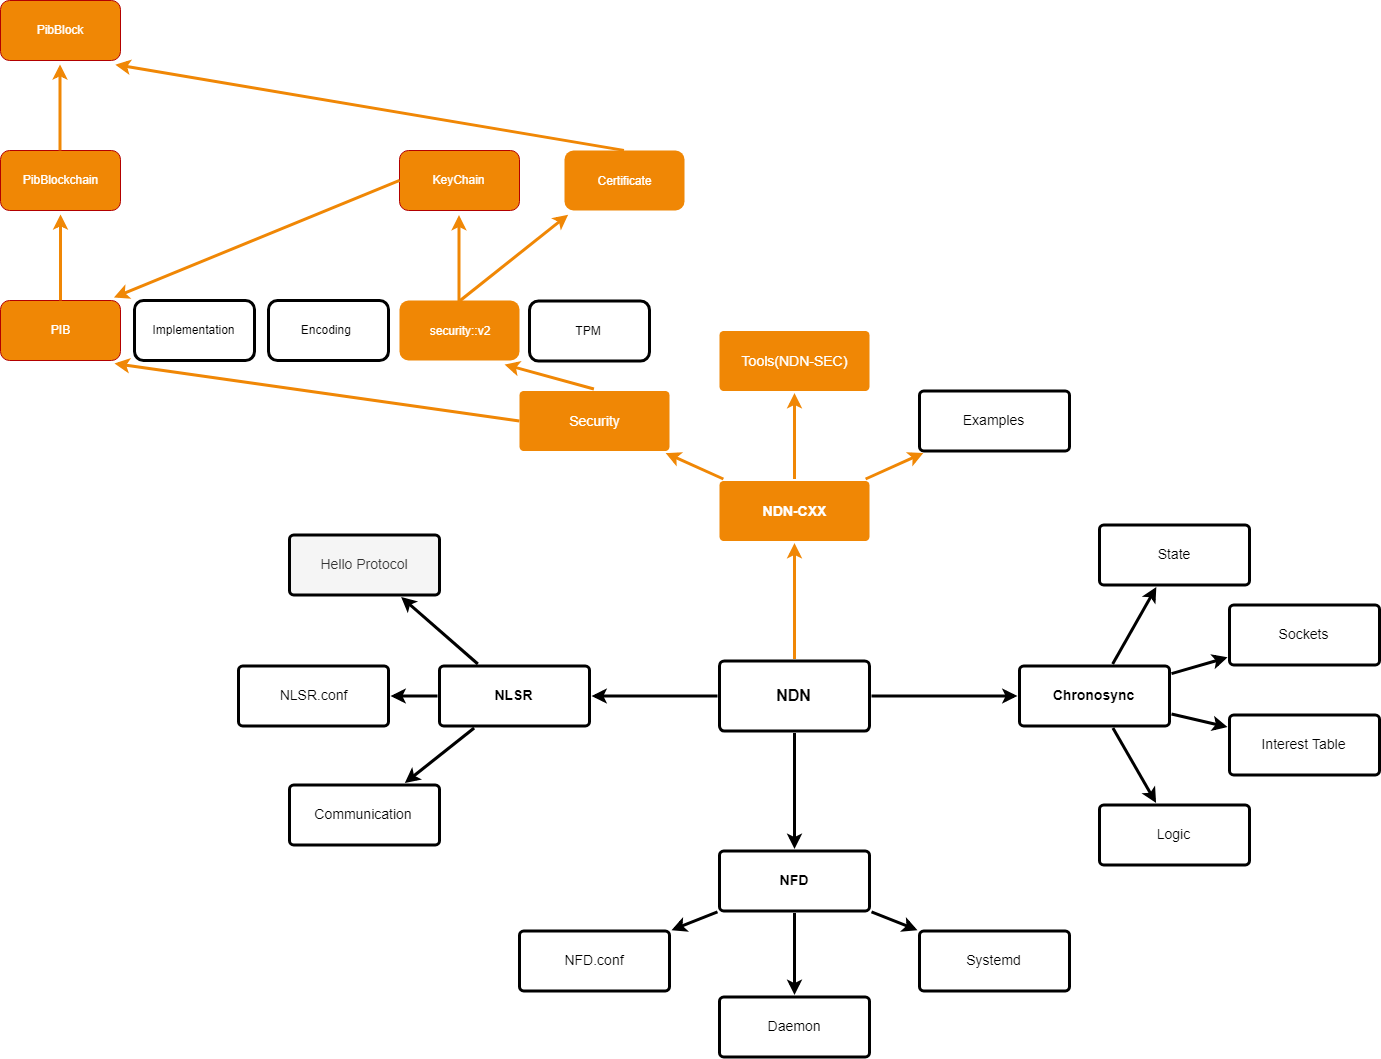
\includegraphics[width=6in]{NDN.png}
\caption{
NDN Components.Orange Rectangles - Intimate knowledge of modules' code required. Orange Rectangles w/ Red Frames - Modules where code was either altered or added for the scope of this project.}
\end{figure}